\documentclass[tikz]{standalone}
\usepackage{amsmath,amssymb}
\usepackage{tikz}
\usetikzlibrary{
	shapes,
	snakes,
	calc,
	decorations,
	decorations.markings,
	decorations.text,
	decorations.pathreplacing}
	
\begin{document}
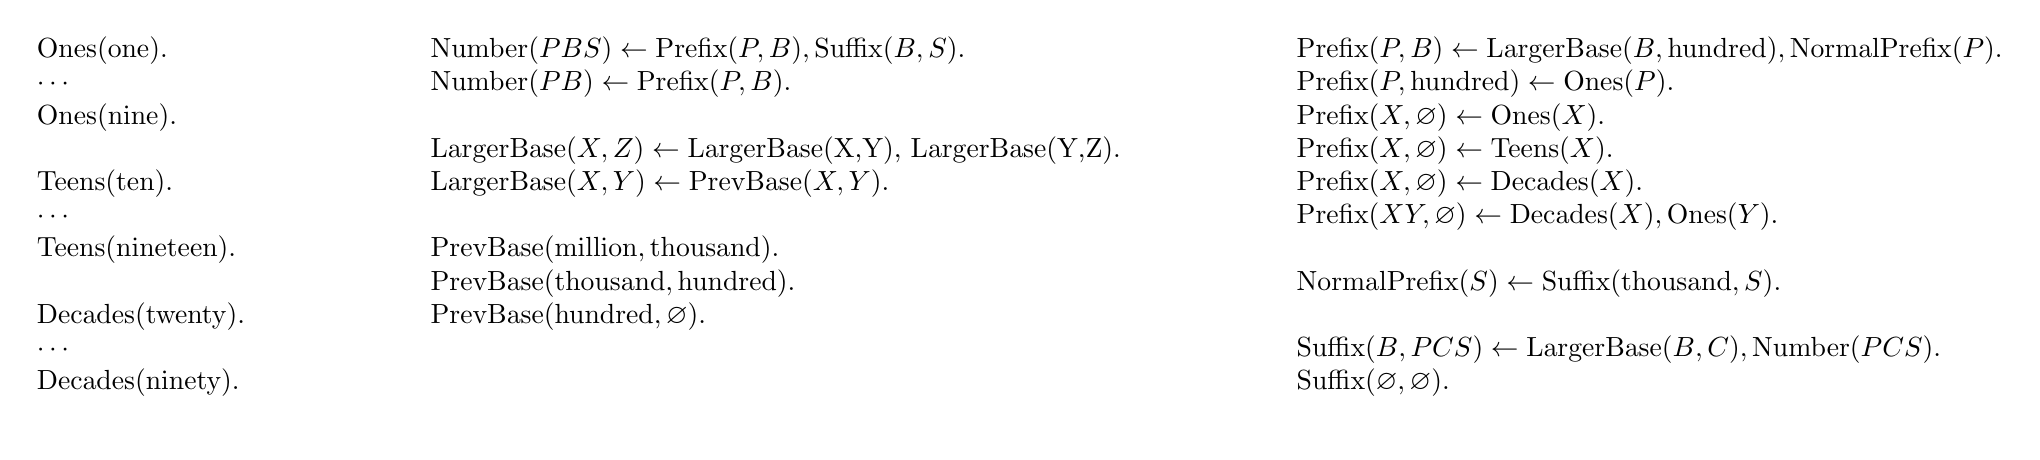
\begin{tikzpicture}[scale=1,every text node part/.style={align=left}]
  \tikzstyle{vertex}=[circle,draw,minimum size=19pt,
    inner sep=1pt, outer sep=1pt]
  
  \node [anchor=north west] (desc) at (0,0) {
    $\text{Ones}(\text{one}).$\\
    $\cdots$\\
    $\text{Ones}(\text{nine}).$\\
    \\
    $\text{Teens}(\text{ten}).$\\
    $\cdots$\\
    $\text{Teens}(\text{nineteen}).$\\
    \\
    $\text{Decades}(\text{twenty}).$\\
    $\cdots$\\
    $\text{Decades}(\text{ninety}).$
  };
  \node [anchor=north west] (desc) at (5,0) {
    $\text{Number}(P B S) \leftarrow \text{Prefix}(P,B), \text{Suffix}(B,S).$\\
    $\text{Number}(P B) \leftarrow \text{Prefix}(P,B).$\\
    \\
    $\text{LargerBase}(X,Z) \leftarrow \text{LargerBase(X,Y), LargerBase(Y,Z).}$\\
    $\text{LargerBase}(X,Y) \leftarrow \text{PrevBase}(X,Y).$\\
    \\
    $\text{PrevBase}(\text{million}, \text{thousand}).$\\
    $\text{PrevBase}(\text{thousand}, \text{hundred}).$\\
    $\text{PrevBase}(\text{hundred}, \varnothing).$
  };
  \node [anchor=north west] (desc) at (16,0) {
    $\text{Prefix}(P,B) \leftarrow \text{LargerBase}(B,\text{hundred}), \text{NormalPrefix}(P).$\\
    $\text{Prefix}(P,\text{hundred}) \leftarrow \text{Ones}(P).$\\
    $\text{Prefix}(X, \varnothing) \leftarrow \text{Ones}(X).$\\
    $\text{Prefix}(X, \varnothing) \leftarrow \text{Teens}(X).$\\
    $\text{Prefix}(X, \varnothing) \leftarrow \text{Decades}(X).$\\
    $\text{Prefix}(X Y, \varnothing) \leftarrow \text{Decades}(X), \text{Ones}(Y).$\\    \\
    $\text{NormalPrefix}(S) \leftarrow \text{Suffix}(\text{thousand},S).$\\
    \\
    $\text{Suffix}(B,PCS) \leftarrow \text{LargerBase}(B,C), \text{Number}(PCS).$\\
    $\text{Suffix}(\varnothing, \varnothing).$\\

  };
\end{tikzpicture}
\end{document}
